\section{Actividad No 04 – CUARTO LATEX AGREGADO} 
		
Nombre : Fiorella Salamanca Contreras\\

\begin{itemize} % CREA GUIONES
\item \textbf{¿Que es GitHub?}\\

GitHub es un servicio de alojamiento web para proyectos que utilizan el sistema de control de revisiones Pequeño icono de GitGit . Está escrito en Ruby on Rails por los desarrolladores de Logical Awesome Chris Wanstrath, PJ Hyett y Tom Preston-Werner. GitHub ofrece planes comerciales y cuentas gratuitas para proyectos de código abierto.

El sitio proporciona funciones de redes sociales como una alimentacion de contenido, seguidores y el gráfico de red para mostrar cómo los desarrolladores trabajan en sus versiones de un repositorio.

Otros autores lo señalan como una plataforma de desarrollo colaborativo de software para alojar proyectos utilizando el sistema de control de versiones Git,debido a que el código se almacena de forma pública, aunque también se puede hacer de forma privada, creando una cuenta de pago.\\

\begin{center}

\includegraphics[width=6cm]{./Imagenes/actividad0401} 
\end{center}
	
\end{itemize} 


\begin{itemize} % CREA GUIONES
\item \textbf{¿Porque es importante GitHub?}\\

GitHub permite alojar en tu repositorio el código de desarrollo de proyecto y te brinda herramientas muy útiles para el trabajo en equipo, dentro de un proyecto.

Además de eso, puedes contribuir a mejorar el software de los demás. Para poder alcanzar esta meta, GitHub provee de funcionalidades para hacer un fork y solicitar pulls.

Realizar un fork es simplemente clonar un repositorio ajeno (genera una copia en tu cuenta), para eliminar algún bug o modificar cosas de él. Una vez realizadas tus modificaciones puedes enviar un pull al dueño del proyecto. Éste podrá analizar los cambios que has realizado fácilmente, y si considera interesante tu contribución, adjuntarlo con el repositorio original.\\

\begin{center}
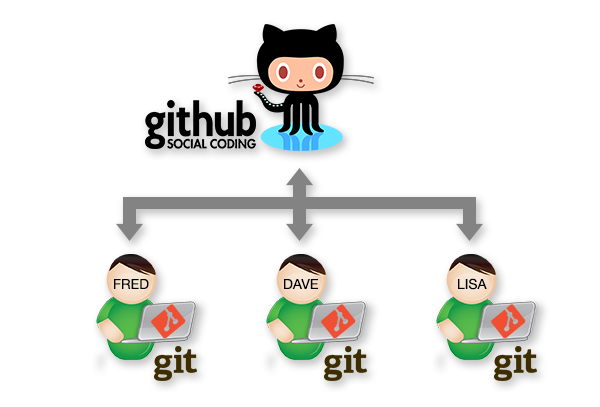
\includegraphics[width=12cm]{./Imagenes/actividad0402} 
\end{center}
	
\end{itemize} 
